\documentclass{article}
\usepackage[utf8]{inputenc}
\usepackage[english]{babel}
\usepackage{multicol}
\usepackage{graphicx}
\graphicspath{ {./figs/} }
\usepackage[a4paper, total={6in, 8in}]{geometry}
\setlength{\parskip}{1em}

\title{Midterm Project Report, Bayes Rules Classifier}
\author{Tao(Richie) Lin}
\date{\today}


\begin{document}
\maketitle
\begin{multicols}{2}
\section{Abstract}
This paper is an experiment report from the Machine Learning class with Professor Haralick. By researching, designing, and implementing the experiment, the goal is to understand better the mechanism, application, and limitation of the Bayes rule classifier.
The experiment was divided into three major parts: 1) design a generator that creates a random multinomial one-dimensional array. The measurement of space and the class will be made from this array. 2) design a series of programs that implement the Bayes rule classifier with economic gain. 3) design an optimization process and evaluate the result.
The result shows that the Bayes conditional probability has a strong correlation to the class having the highest probability when the data is randomly generated. The optimization has small or no impact on the scenario that the score of incorrect assignment is higher than the correct ones in the economic gain matrix. 
\section{Introduction}
As an extremely important component of modern statistics, Bayes Theorem has provided a powerful angle looking at the world with the conditional probability. Additional to the contribution to the statistics, it is also a widely used algorithm in the field of machine learning. In the class of Machine Learning, Professor Haralick has instructed us to accomplish a series of experiments, including understanding the theory of Bayes Theorem, design the experiment procedures, implementing the coding process, evaluating the result.
\section{Experiment Process}
As a person who started building skillsets from statistical programming, my primary programming language is R. when working on this project. There are a couple of built-in functions in R that provided the short cuts to accomplish the functions that might need a lot of additional steps to do, such as generating uniformly distributed arrays, vectorized computation instead of interactive computation, and Boolean masking subsetting instead of iterative comparison.
The experiment was completed in three major steps: generating random multinominal datasets for training and testing; building a program that calculates the expectation of the economic gain based on the Bayes rule; Optimization by adding the marginal change on the correct assignment for a set number of iterations.
As one of the characteristic logics in R programming or any statistics programming language, it would be easier to manipulate a dataset rather than building the program from zero. In such a case, I started with making the synthetic dataset generator. 
\subsection{Building synthetic dataset generator}
The synthetic dataset generator is designed to generate a random one-dimensional array with two core parameters: the number of possible values (or class if generating the dependent variable) and the number of observations.
The number of possible values Y is used to generate a uniformly distributed array with the range from 0 to 1. The total number of elements in Y. We normalized the array by dividing each element by the sum of them. We fed it into a loop to calculate an array of cumulative probability. The newly generated array will be used as the upper limit of the category. 

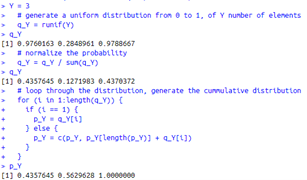
\includegraphics{fig1.png}

In the screenshot of $n$ example above, the total number of element $Y$ was set as 3. The uniform distributed array q\_Y has a value of 0.9356429, 0.6021019, and 0.4127837. By dividing the sum of all of them, the normalized array has the values of 0.4357645, 0.1271983, 0.4370372. Finally, the cumulative distribution calculated from the loop is 0.4357645, 0.5629628, 1.0000000, which serves as the upper limit of each assignment window.
The next step is to input the number of observations, size and generated a uniformly distributed array, d, with the range from 0 to 1 and total elements as size.
Each element of d will be fed into a loop of comparison with the values p\_Y. In the example of the screenshot above, if the values are greater than 0 but smaller or equal to 4.357645, the label of this element will be assigned as 1; if it is great than the previous upper limit and smaller than 0.5629628, the label will be assigned as 2; same applies to the third circumstances, which the label of the element will be assigned as 3.
When the iteration is completed, we will have a one-dimensional array with the possible number value of Y, and the total number of the element as size, the probability of each label being assigned is p\_Y.
However, as a relatively high level of programming language, R provides a vectorized computational logic, which allows users to apply the manipulation on the entire array level rather than looping through each of them. That character makes our functions hit the performance issue when the size was set more than 1 million. However, when the number of observations in the measurement space was not big enough (in my case, I would prefer to set it at 3 million), some x tuple would not have enough samples to calculate a meaningful prior conditional probability. In such consideration, I decided to go ahead and use one of the powerful preset functions in R: sample(). It generates a randomly distributed one-dimensional array when the given number of possible values of labels, number of observations, and the probability of each possible values. 

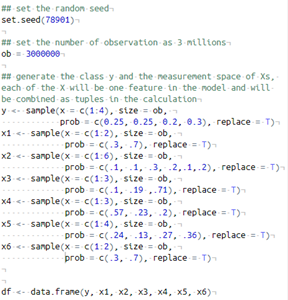
\includegraphics{fig2.png}

In the screenshot above, I generated a measurement space with six features: x1 – x6 with the same number of observations but different numbers and probability of the possible labels. They are combined in a data frame with the true class array y.
\subsection{Calculating Bayes rule}
From the slides, I learned to form the professor that the Bayes rules that are more generally applicable to real-world problem solving are considering the economics gains for every assignment. It was a fascinating idea to me and elevated my level of thinking in applying machine learning techniques in real-world problem-solving. 
So in building the Bayes rules, I divided the constructions into three parts: 
\begin{itemize}
\item Building a function that calculates the prior conditional probability $P(d|c)$ and the class probability $P(c)$;
\item Building a function that calculates the Bayes posterior conditional probability $P(c|d)$
\item Multiply the economics gain to each assignment class's probability for every x tuple for the economic gains.
\end{itemize}
Before building these functions, I divided the dataset into a training set and testing set. 

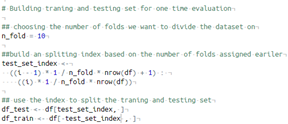
\includegraphics{fig3.png}

This step, by providing the number of folds wanted, calculates the staring row and the ending row and saves it as a test set index. We can use the Boolean mask feature in R programming to subset the index's training set and testing set.
The function that calculates the prior conditional probability is called fun\_prob() in my code. It takes a data frame with columns named Xn and Y and produces the table that contains the prior probability of each x tuple in every given y.

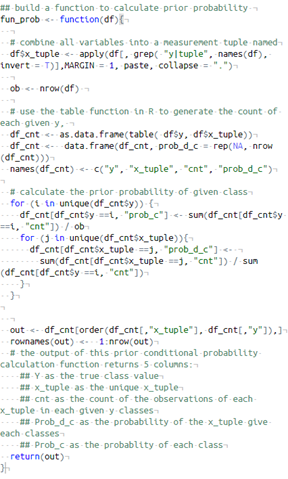
\includegraphics{fig4.png}

The first step is to convert the measurement space to an x tiple by combining all measurement features Xs. There is a handy function called paste(), which string all elements into one string in R. Using the apply() function to cast the paste() on all the elements in each feature, it produces the x tuple with all features combined.
Rather than counting the number of appearances in a loop, R has a great function table(), which produces the count of each unique x tuple. When given the second element to the function, in our case, the true class label y, it can also produce the crosstab of x tuples and y. the result is shown below.

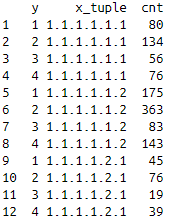
\includegraphics{fig5.png}

Using the count from the crosstab, the conditional probability can be easily calculated simply by dividing each true class label's total count. Here is an example of the output:

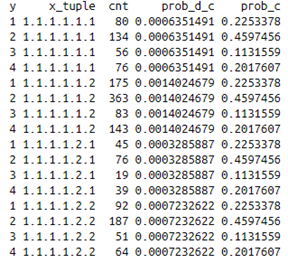
\includegraphics{fig6.png}

This function is very useful to produce the elements in the Bayes theorem:

$P(c_n|d)= \frac{P(d | c)P(c)}{P(d,c)} = \frac{P(d | c)P(c)}{\sum_{n=1}^k P(d|c_n)P(c_n))}$

The numerator and denominator element in the expanded form of this conditional probability can be calculated with the function.
Build the function to calculate the posterior conditional probability with the economic gain.
Based on the Bayes conditional probability:

$P(c_n|d)= \frac{P(d | c)P(c)}{P(d,c)} = \frac{P(d | c)P(c)}{\sum_{n=1}^k P(d|c_n)P(c_n))}$

To calculate each possible assignment class's probability, we need to use the conditional probability multiply the class probability that we wanted to calculate from the training set in the numerator. The denominator would be the joint probability of all possible true class and the conditional probability of the x tuple from the testing set. 

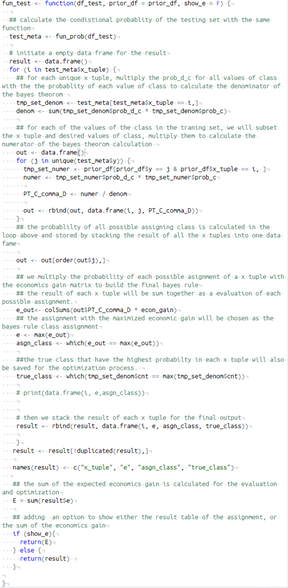
\includegraphics{fig7.png}

Because the testing set is involved in this calculation step, I named it fun\_test(). The first step in this function is to calculate the conditional probability of the testing set. It can be done easily with the function we built earlier. 
A nested loop is then used to calculate each possible class assignment's probability on each x tuples. Firstly loop through all the x tuples, subset the conditional probability from the training set to calculate the denominator as shared in the calculation in all possible, then loop through y to calculate the numerator in calculating the probability for each possible assignable class. 

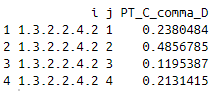
\includegraphics{fig8.png}

The screenshot above is the calculation result of the x tuple 1.3.2.2.4.2, given the possible assignment class 1,2,3 and 4.
After stacking up the results for each possible assignment class, we multiply the array of probability to the economic gain matrix. 

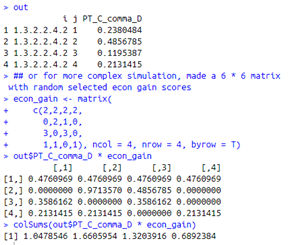
\includegraphics{fig9.png}

By summing up the economic gain, we chose the assignment with the highest overall economic gain. In the example shown above, each possible assignment's economic gain was calculated as 1.04, 1.66, 1.32, and 0.69. in the example above, the x tuple of 1.3.2.2.4.2 will be assigned to class 2 for having the highest economic gain.
After calculating the economic gain for all x tuples, we store the assigned class and the true class, which has the highest P (d |c) probability for the optimization process. Along with these probabilities, we also sum the total economic gain for all x tuples for the evaluation.
The result set of the function looks like the screenshot below:

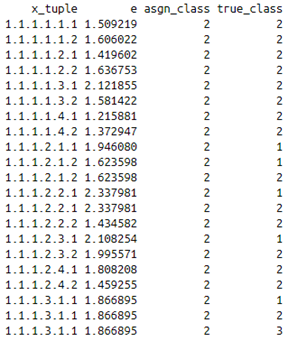
\includegraphics{fig10.png}

Most of the x tuple in the example above got assigned as class 2 because the overall probability of class 2 is the highest (0.4596163 vs. 0.2251065, 0.1132197, and 0.2020574) also. In the economic gain matrix, the reward of assigning it to class 2 is also pretty high.
\subsection{Optimization}
The assignment could be rewarded by setting a marginal change value and adding it to the correct assignment's conditional probability, thus further optimized.
Here is an example code of optimization In my experiment:

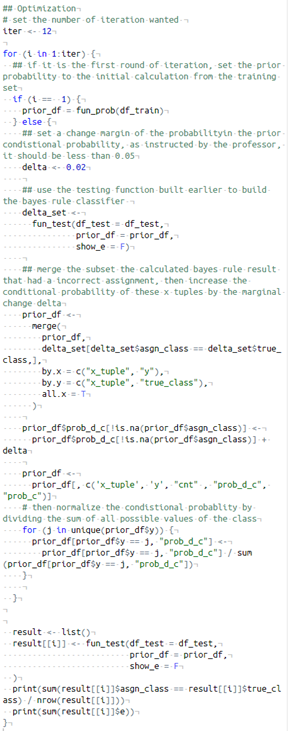
\includegraphics{fig11.png}

First, set a number of iteration. I choose 12 because it reaches the max expected gain after several rounds of experiments. 
For the first round of the iteration, the prior conditional probability is calculated with the function built earlier.
For each round of iteration following, the prior conditional probability is inherited from the previous round. 
By looking at only the correct assignment from the Bayes rule assignment result, we can now target the x tuple and the correctly assigned y class. Merge the subset with the prior probability table as a filter, add the delta to the prior conditional probability, and then normalize it to make the probability of given x tuple in all y classes sum to 1. 
By doing so, the correct assignment will be rewarded by the marginal value in each iteration. 

Here we have completed the experiment with the Bayes rule classifier.
\section{Experimental Result \& Conclusions}
\begin{enumerate}
    \item When all the variables were randomly generated and uniformly distributed, the calculated posterior conditional distribution will have a strong correlation with the true class with the highest probability.
    \item Because each of the x tuples can be assigned to only one class when the dataset is randomly uniformly distributed, the maximum correct assignment rate would never reach 100%, regardless of how many rounds of optimization was used.
    \item Though the correct identification rate's peak will be reached after a few iterations of the optimization process, the expected gain's peak will continue to grow. The optimization result below was from a Bayes rule classifier with the economics gain as an identity matrix with dimensions equals the number of possible classes.
    
    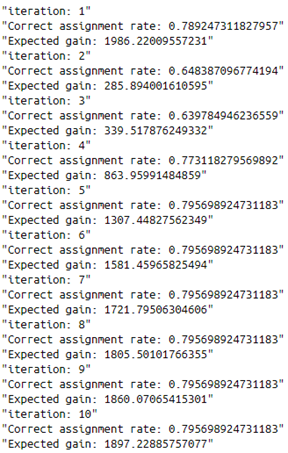
\includegraphics{fig12.png}

    \item The economic gain has a significant impact on the assignment. When rewarding the incorrect assignment is multiple times bigger than the correct assignment, it could potentially impair the optimization for the correct assignment rate. Show as the example below:  
    
    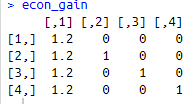
\includegraphics{fig13.png} 

    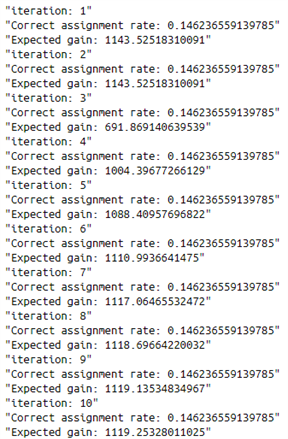
\includegraphics{fig14.png}
    
\end{enumerate}
\end{multicols}
\end{document}
